\documentclass{extbook}[14pt]
\usepackage{multicol, enumerate, enumitem, hyperref, color, soul, setspace, parskip, fancyhdr, amssymb, amsthm, amsmath, latexsym, units, mathtools}
\everymath{\displaystyle}
\usepackage[headsep=0.5cm,headheight=0cm, left=1 in,right= 1 in,top= 1 in,bottom= 1 in]{geometry}
\usepackage{dashrule}  % Package to use the command below to create lines between items
\newcommand{\litem}[1]{\item #1

\rule{\textwidth}{0.4pt}}
\pagestyle{fancy}
\lhead{}
\chead{Answer Key for Progress Quiz 8 Version B}
\rhead{}
\lfoot{5493-4176}
\cfoot{}
\rfoot{Summer C 2021}
\begin{document}
\textbf{This key should allow you to understand why you choose the option you did (beyond just getting a question right or wrong). \href{https://xronos.clas.ufl.edu/mac1105spring2020/courseDescriptionAndMisc/Exams/LearningFromResults}{More instructions on how to use this key can be found here}.}

\textbf{If you have a suggestion to make the keys better, \href{https://forms.gle/CZkbZmPbC9XALEE88}{please fill out the short survey here}.}

\textit{Note: This key is auto-generated and may contain issues and/or errors. The keys are reviewed after each exam to ensure grading is done accurately. If there are issues (like duplicate options), they are noted in the offline gradebook. The keys are a work-in-progress to give students as many resources to improve as possible.}

\rule{\textwidth}{0.4pt}

\begin{enumerate}\litem{
Construct the lowest-degree polynomial given the zeros below. Then, choose the intervals that contain the coefficients of the polynomial in the form $ax^3+bx^2+cx+d$.
\[ \frac{-7}{4}, -1, \text{ and } -3 \]The solution is \( 4x^{3} +23 x^{2} +40 x + 21 \), which is option B.\begin{enumerate}[label=\Alph*.]
\item \( a \in [2, 5], b \in [21, 29], c \in [37, 41], \text{ and } d \in [-23, -18] \)

$4x^{3} +23 x^{2} +40 x -21$, which corresponds to multiplying everything correctly except the constant term.
\item \( a \in [2, 5], b \in [21, 29], c \in [37, 41], \text{ and } d \in [20, 22] \)

* $4x^{3} +23 x^{2} +40 x + 21$, which is the correct option.
\item \( a \in [2, 5], b \in [-24, -16], c \in [37, 41], \text{ and } d \in [-23, -18] \)

$4x^{3} -23 x^{2} +40 x -21$, which corresponds to multiplying out $(4x -7)(x -1)(x -3)$.
\item \( a \in [2, 5], b \in [6, 12], c \in [-19, -11], \text{ and } d \in [-23, -18] \)

$4x^{3} +9 x^{2} -16 x -21$, which corresponds to multiplying out $(4x -7)(x + 1)(x + 3)$.
\item \( a \in [2, 5], b \in [0, 3], c \in [-33, -25], \text{ and } d \in [20, 22] \)

$4x^{3} + x^{2} -26 x + 21$, which corresponds to multiplying out $(4x -7)(x -1)(x + 3)$.
\end{enumerate}

\textbf{General Comment:} To construct the lowest-degree polynomial, you want to multiply out $(4x + 7)(x + 1)(x + 3)$
}
\litem{
Describe the end behavior of the polynomial below.
\[ f(x) = 5(x + 4)^{2}(x - 4)^{3}(x + 8)^{5}(x - 8)^{6} \]The solution is the graph below, which is option C.
    \begin{center}
        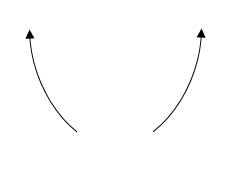
\includegraphics[width=0.3\textwidth]{../Figures/polyEndBehaviorCopyCB.png}
    \end{center}\begin{enumerate}[label=\Alph*.]
\begin{multicols}{2}
\item 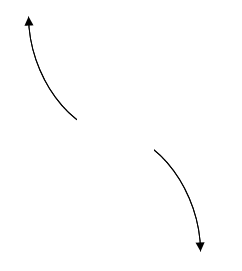
\includegraphics[width = 0.3\textwidth]{../Figures/polyEndBehaviorCopyAB.png}
\item 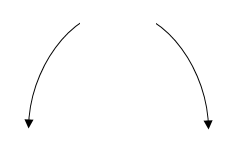
\includegraphics[width = 0.3\textwidth]{../Figures/polyEndBehaviorCopyBB.png}
\item 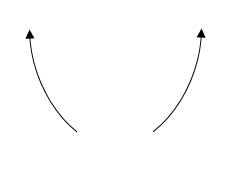
\includegraphics[width = 0.3\textwidth]{../Figures/polyEndBehaviorCopyCB.png}
\item 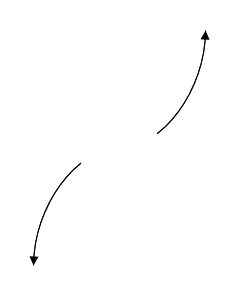
\includegraphics[width = 0.3\textwidth]{../Figures/polyEndBehaviorCopyDB.png}
\end{multicols}\item None of the above.\end{enumerate}
\textbf{General Comment:} Remember that end behavior is determined by the leading coefficient AND whether the \textbf{sum} of the multiplicities is positive or negative.
}
\litem{
Construct the lowest-degree polynomial given the zeros below. Then, choose the intervals that contain the coefficients of the polynomial in the form $x^3+bx^2+cx+d$.
\[ 4 - 5 i \text{ and } 4 \]The solution is \( x^{3} -12 x^{2} +73 x -164 \), which is option A.\begin{enumerate}[label=\Alph*.]
\item \( b \in [-13, -11], c \in [71, 74], \text{ and } d \in [-171, -156] \)

* $x^{3} -12 x^{2} +73 x -164$, which is the correct option.
\item \( b \in [9, 15], c \in [71, 74], \text{ and } d \in [156, 167] \)

$x^{3} +12 x^{2} +73 x + 164$, which corresponds to multiplying out $(x-(4 - 5 i))(x-(4 + 5 i))(x + 4)$.
\item \( b \in [-6, 2], c \in [-11, -2], \text{ and } d \in [16, 20] \)

$x^{3} + x^{2} -8 x + 16$, which corresponds to multiplying out $(x -4)(x -4)$.
\item \( b \in [-6, 2], c \in [-1, 11], \text{ and } d \in [-28, -19] \)

$x^{3} + x^{2} +x -20$, which corresponds to multiplying out $(x + 5)(x -4)$.
\item \( \text{None of the above.} \)

This corresponds to making an unanticipated error or not understanding how to use nonreal complex numbers to create the lowest-degree polynomial. If you chose this and are not sure what you did wrong, please contact the coordinator for help.
\end{enumerate}

\textbf{General Comment:} Remember that the conjugate of $a+bi$ is $a-bi$. Since these zeros always come in pairs, we need to multiply out $(x-(4 - 5 i))(x-(4 + 5 i))(x-(4))$.
}
\litem{
Describe the end behavior of the polynomial below.
\[ f(x) = -2(x + 7)^{3}(x - 7)^{4}(x - 8)^{3}(x + 8)^{5} \]The solution is the graph below, which is option A.
    \begin{center}
        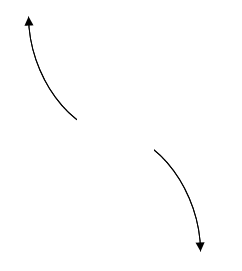
\includegraphics[width=0.3\textwidth]{../Figures/polyEndBehaviorAB.png}
    \end{center}\begin{enumerate}[label=\Alph*.]
\begin{multicols}{2}
\item 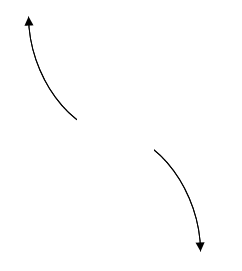
\includegraphics[width = 0.3\textwidth]{../Figures/polyEndBehaviorAB.png}
\item 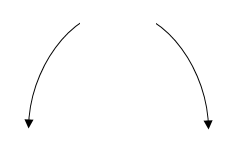
\includegraphics[width = 0.3\textwidth]{../Figures/polyEndBehaviorBB.png}
\item 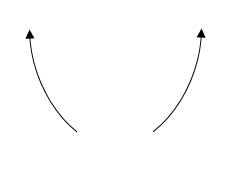
\includegraphics[width = 0.3\textwidth]{../Figures/polyEndBehaviorCB.png}
\item 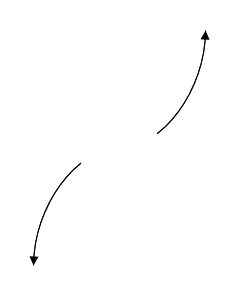
\includegraphics[width = 0.3\textwidth]{../Figures/polyEndBehaviorDB.png}
\end{multicols}\item None of the above.\end{enumerate}
\textbf{General Comment:} Remember that end behavior is determined by the leading coefficient AND whether the \textbf{sum} of the multiplicities is positive or negative.
}
\litem{
Which of the following equations \textit{could} be of the graph presented below?

\begin{center}
    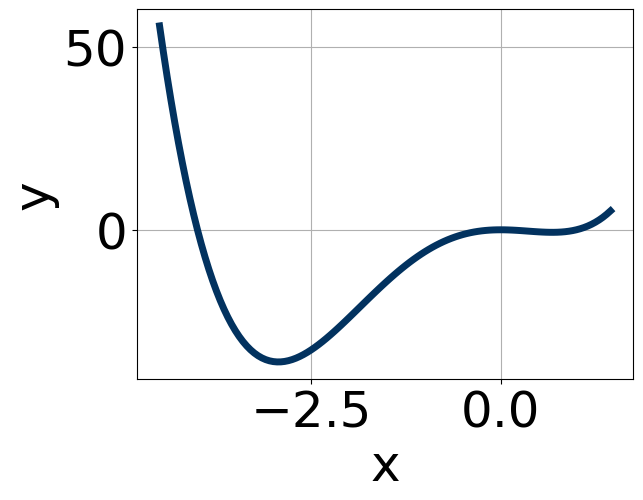
\includegraphics[width=0.5\textwidth]{../Figures/polyGraphToFunctionCopyB.png}
\end{center}


The solution is \( 16x^{10} (x - 1)^{5} (x + 4)^{9} \), which is option B.\begin{enumerate}[label=\Alph*.]
\item \( -7x^{10} (x - 1)^{9} (x + 4)^{8} \)

The factor $(x + 4)$ should have an odd power and the leading coefficient should be the opposite sign.
\item \( 16x^{10} (x - 1)^{5} (x + 4)^{9} \)

* This is the correct option.
\item \( -12x^{8} (x - 1)^{9} (x + 4)^{9} \)

This corresponds to the leading coefficient being the opposite value than it should be.
\item \( 13x^{10} (x - 1)^{8} (x + 4)^{11} \)

The factor $(x - 1)$ should have an odd power.
\item \( 4x^{5} (x - 1)^{6} (x + 4)^{9} \)

The factor $0$ should have an even power and the factor $1$ should have an odd power.
\end{enumerate}

\textbf{General Comment:} General Comments: Draw the x-axis to determine which zeros are touching (and so have even multiplicity) or cross (and have odd multiplicity).
}
\litem{
Describe the zero behavior of the zero $x = -7$ of the polynomial below.
\[ f(x) = -5(x - 2)^{6}(x + 2)^{4}(x + 7)^{6}(x - 7)^{5} \]The solution is the graph below, which is option C.
    \begin{center}
        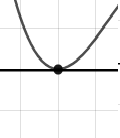
\includegraphics[width=0.3\textwidth]{../Figures/polyZeroBehaviorCB.png}
    \end{center}\begin{enumerate}[label=\Alph*.]
\begin{multicols}{2}
\item 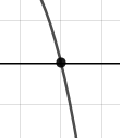
\includegraphics[width = 0.3\textwidth]{../Figures/polyZeroBehaviorAB.png}
\item 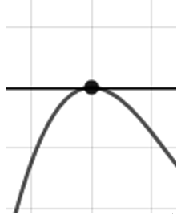
\includegraphics[width = 0.3\textwidth]{../Figures/polyZeroBehaviorBB.png}
\item 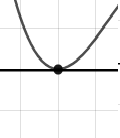
\includegraphics[width = 0.3\textwidth]{../Figures/polyZeroBehaviorCB.png}
\item 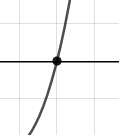
\includegraphics[width = 0.3\textwidth]{../Figures/polyZeroBehaviorDB.png}
\end{multicols}\item None of the above.\end{enumerate}
\textbf{General Comment:} You will need to sketch the entire graph, then zoom in on the zero the question asks about.
}
\litem{
Construct the lowest-degree polynomial given the zeros below. Then, choose the intervals that contain the coefficients of the polynomial in the form $x^3+bx^2+cx+d$.
\[ -3 + 2 i \text{ and } -4 \]The solution is \( x^{3} +10 x^{2} +37 x + 52 \), which is option A.\begin{enumerate}[label=\Alph*.]
\item \( b \in [10, 19], c \in [32, 39], \text{ and } d \in [51, 63] \)

* $x^{3} +10 x^{2} +37 x + 52$, which is the correct option.
\item \( b \in [-1, 3], c \in [4, 8], \text{ and } d \in [11, 17] \)

$x^{3} + x^{2} +7 x + 12$, which corresponds to multiplying out $(x + 3)(x + 4)$.
\item \( b \in [-1, 3], c \in [-4, 3], \text{ and } d \in [-12, -5] \)

$x^{3} + x^{2} +2 x -8$, which corresponds to multiplying out $(x -2)(x + 4)$.
\item \( b \in [-11, -7], c \in [32, 39], \text{ and } d \in [-52, -50] \)

$x^{3} -10 x^{2} +37 x -52$, which corresponds to multiplying out $(x-(-3 + 2 i))(x-(-3 - 2 i))(x -4)$.
\item \( \text{None of the above.} \)

This corresponds to making an unanticipated error or not understanding how to use nonreal complex numbers to create the lowest-degree polynomial. If you chose this and are not sure what you did wrong, please contact the coordinator for help.
\end{enumerate}

\textbf{General Comment:} Remember that the conjugate of $a+bi$ is $a-bi$. Since these zeros always come in pairs, we need to multiply out $(x-(-3 + 2 i))(x-(-3 - 2 i))(x-(-4))$.
}
\litem{
Construct the lowest-degree polynomial given the zeros below. Then, choose the intervals that contain the coefficients of the polynomial in the form $ax^3+bx^2+cx+d$.
\[ \frac{7}{5}, \frac{-5}{2}, \text{ and } \frac{1}{2} \]The solution is \( 20x^{3} +12 x^{2} -81 x + 35 \), which is option B.\begin{enumerate}[label=\Alph*.]
\item \( a \in [18, 21], b \in [65, 73], c \in [23, 32], \text{ and } d \in [-35, -33] \)

$20x^{3} +68 x^{2} +31 x -35$, which corresponds to multiplying out $(5x + 7)(2x + 5)(2x -1)$.
\item \( a \in [18, 21], b \in [8, 17], c \in [-95, -77], \text{ and } d \in [33, 37] \)

* $20x^{3} +12 x^{2} -81 x + 35$, which is the correct option.
\item \( a \in [18, 21], b \in [8, 17], c \in [-95, -77], \text{ and } d \in [-35, -33] \)

$20x^{3} +12 x^{2} -81 x -35$, which corresponds to multiplying everything correctly except the constant term.
\item \( a \in [18, 21], b \in [-33, -27], c \in [-68, -57], \text{ and } d \in [33, 37] \)

$20x^{3} -32 x^{2} -59 x + 35$, which corresponds to multiplying out $(5x + 7)(2x -5)(2x -1)$.
\item \( a \in [18, 21], b \in [-18, -3], c \in [-95, -77], \text{ and } d \in [-35, -33] \)

$20x^{3} -12 x^{2} -81 x -35$, which corresponds to multiplying out $(5x + 7)(2x -5)(2x + 1)$.
\end{enumerate}

\textbf{General Comment:} To construct the lowest-degree polynomial, you want to multiply out $(5x -7)(2x + 5)(2x -1)$
}
\litem{
Which of the following equations \textit{could} be of the graph presented below?

\begin{center}
    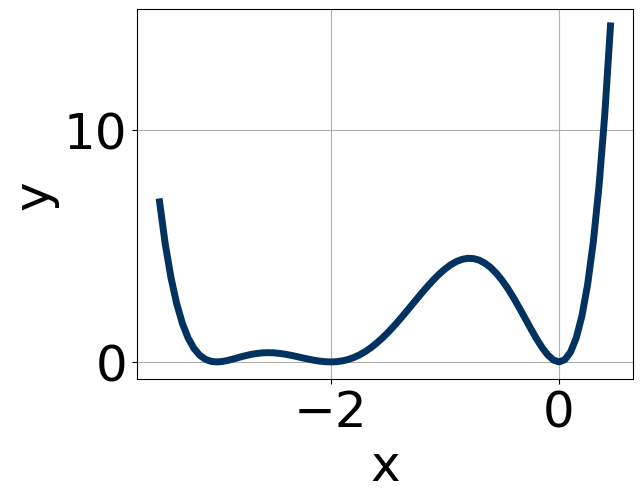
\includegraphics[width=0.5\textwidth]{../Figures/polyGraphToFunctionB.png}
\end{center}


The solution is \( 8x^{6} (x + 3)^{10} (x + 2)^{10} \), which is option D.\begin{enumerate}[label=\Alph*.]
\item \( 14x^{11} (x + 3)^{6} (x + 2)^{7} \)

The factors $x$ and $(x + 2)$ should both have even powers.
\item \( 16x^{10} (x + 3)^{4} (x + 2)^{11} \)

The factor $(x + 2)$ should have an even power.
\item \( -4x^{8} (x + 3)^{8} (x + 2)^{4} \)

This corresponds to the leading coefficient being the opposite value than it should be.
\item \( 8x^{6} (x + 3)^{10} (x + 2)^{10} \)

* This is the correct option.
\item \( -5x^{8} (x + 3)^{6} (x + 2)^{7} \)

The factor $(x + 2)$ should have an even power and the leading coefficient should be the opposite sign.
\end{enumerate}

\textbf{General Comment:} General Comments: Draw the x-axis to determine which zeros are touching (and so have even multiplicity) or cross (and have odd multiplicity).
}
\litem{
Describe the zero behavior of the zero $x = 9$ of the polynomial below.
\[ f(x) = -3(x + 9)^{6}(x - 9)^{11}(x - 5)^{8}(x + 5)^{9} \]The solution is the graph below, which is option A.
    \begin{center}
        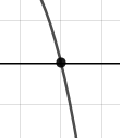
\includegraphics[width=0.3\textwidth]{../Figures/polyZeroBehaviorCopyAB.png}
    \end{center}\begin{enumerate}[label=\Alph*.]
\begin{multicols}{2}
\item 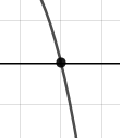
\includegraphics[width = 0.3\textwidth]{../Figures/polyZeroBehaviorCopyAB.png}
\item 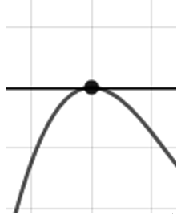
\includegraphics[width = 0.3\textwidth]{../Figures/polyZeroBehaviorCopyBB.png}
\item 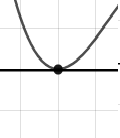
\includegraphics[width = 0.3\textwidth]{../Figures/polyZeroBehaviorCopyCB.png}
\item 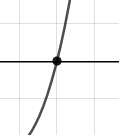
\includegraphics[width = 0.3\textwidth]{../Figures/polyZeroBehaviorCopyDB.png}
\end{multicols}\item None of the above.\end{enumerate}
\textbf{General Comment:} You will need to sketch the entire graph, then zoom in on the zero the question asks about.
}
\end{enumerate}

\end{document}